\begin{figure}[H]
\centering
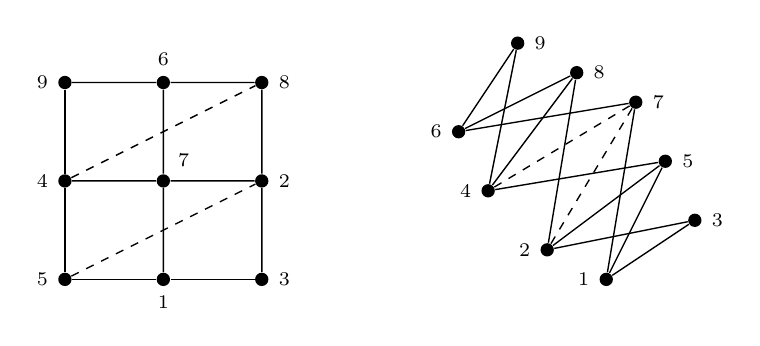
\begin{tikzpicture}[
    scale=1.25,
    vertex/.style={circle, fill=black, inner sep=1.7pt},
    edge/.style={line width=0.5pt}
]

% Left column: embedding
\begin{scope}[xshift=0cm]
    \node[vertex, label={[font=\scriptsize]left:9}] (a) at (0,2) {};
    \node[vertex, label={[font=\scriptsize]above:6}] (b) at (1,2) {};
    \node[vertex, label={[font=\scriptsize]right:8}] (c) at (2,2) {};

    \node[vertex, label={[font=\scriptsize]left:4}] (d) at (0,1) {};
    \node[vertex, label={[font=\scriptsize]above right:7}] (e) at (1,1) {};
    \node[vertex, label={[font=\scriptsize]right:2}] (f) at (2,1) {};

    \node[vertex, label={[font=\scriptsize]left:5}] (g) at (0,0) {};
    \node[vertex, label={[font=\scriptsize]below:1}] (h) at (1,0) {};
    \node[vertex, label={[font=\scriptsize]right:3}] (i) at (2,0) {};

    \draw[edge] (a) -- (d) -- (g);
    \draw[edge] (b) -- (e) -- (h);
    \draw[edge] (c) -- (f) -- (i);

    \draw[edge] (a) -- (b) -- (c);
    \draw[edge] (d) -- (e) -- (f);
    \draw[edge] (g) -- (h) -- (i);

    \draw[edge, dashed] (d) -- (c);
    \draw[edge, dashed] (g) -- (f);
\end{scope}

% Right column: comparability graph
\begin{scope}[xshift=4cm,yscale=1,scale=0.3]
    \node[vertex, label={[font=\scriptsize]right:9}] (a) at (2,8) {};
    \node[vertex, label={[font=\scriptsize]right:8}] (c) at (4,7) {};
    \node[vertex, label={[font=\scriptsize]right:7}] (e) at (6,6) {};
    \node[vertex, label={[font=\scriptsize]left:6}]  (b) at (0,5) {};
    \node[vertex, label={[font=\scriptsize]right:5}] (g) at (7,4) {};
    \node[vertex, label={[font=\scriptsize]left:4}]  (f) at (1,3) {};
    \node[vertex, label={[font=\scriptsize]right:3}] (i) at (8,2) {};
    \node[vertex, label={[font=\scriptsize]left:2}]  (d) at (3,1) {};
    \node[vertex, label={[font=\scriptsize]left:1}]  (h) at (5,0) {};

    \draw[edge] (h) -- (e);
    \draw[edge] (h) -- (g);
    \draw[edge] (h) -- (i);

    \draw[edge] (d) -- (c);
    \draw[edge, dashed] (d) -- (e);
    \draw[edge] (d) -- (g);
    \draw[edge] (d) -- (i);

    \draw[edge] (f) -- (g);
    \draw[edge, dashed] (f) -- (e);
    \draw[edge] (f) -- (c);
    \draw[edge] (f) -- (a);

    \draw[edge] (b) -- (e);
    \draw[edge] (b) -- (c);
    \draw[edge] (b) -- (a);
\end{scope}

\end{tikzpicture}
\caption{The diagonal graph viewed as a grid with additional edges (left) and as a subgraph of $\CGrid$ (right).}
\label{fig:embedding-comparability}
\end{figure}